\documentclass{article}
\usepackage[utf8]{inputenc}
\usepackage{url}
\usepackage{array}
\usepackage{graphics}
\usepackage{tikz}
\usetikzlibrary{positioning}



\title{Accelerating Matrix Multiplication}
\author{Shubham Jain \\ \texttt{ee3160512@iitd.ac.in} \and Vivek Singal \\ \texttt{ee1160421@iitd.ac.in}}
\date{February 17, 2019}

\begin{document}

\maketitle
Convolution is an essential operation in any CNN architecture. Convolution becomes handy by multiplying convolving matrices using Toeplitz\cite{Toeplitz} representation. Simple Matrix multiplication without any optimization requires highly expensive computions i.e. O\((n^2*m^2)\). To counter this problem we propose usage of a couple of  linear algebra libraries in section 1 and parallel threads in section 2, to speed up matrix multiplication calculations. Finally we report the performance comparison of the several tools used by plotting box plot of the execution time for matrices of different sizes in section 3.  
\section{Linear Algebra Libraries}
We used a couple of API's namely OpenBlas and Intel MKL to accelerate matrix multiplication. They tend to perform better than nested loop strategy because they adopt several optimized and threaded routines over linear math kernels, which operate specific to one's processor. 
\newline
As OpenBlas and MKL both use function with same definition for matrix multiplication, include \textit{cblas.h} or \textit{mkl.h} in the cpp file one at a time, for using OpenBlas or MKL library respectively. If both header files are included,  the library with flags mentioned before the other will be used during runtime.        
\subsection{OpenBlas}
We first installed Openblas library from official site\cite{Openblas}. We used \textit{cblas\_sgemm} function of OpenBlas for matrix multiplication of our input Toeplitz matrix with the kernel matrix where both matrices contain values in float. \textit{cblas\_sgemm} requires the two matrices to be fed as vectors thus we need to specify whether the vectors are in column major or row major format. The result matrix is also returned as a vector in same format. While compiling cpp files which use OpenBlas API we need to include the modules and library path as flags, inorder to link the required libraries while function calls.                    
\subsection{Intel MKL}
We installed intel MKL library from their official website\cite{IntelMKL}. This library involves optimizations specific to intel processors. The names and arguments of the functions used for matrix multiplication are same as that of OpenBlas. Appropriate flags needs to be included in the makefile for compiling code that uses mkl functions. 
\section{C++ Parallel Threads}
The basic idea of using parallel thread here is to break the task of matrix multiplication into smaller subtasks and further distribute them among several cores of the system in the form of threads.
\begin{itemize}
\item Matrix multiplication can be broken into independent subtasks involving matrix multiplication of a single row of first matrix with the entire second matrix and then iterating over each row of first matrix. A separate thread is used for each subtask and subsequently the computation from each tread is collected and further joined together to get each element of the resultant matrix. 
\item Another strategy we adopted was to make separate threads for multiplying each row of matrix 1 with each column of matrix 2 and then first iterating over columns of matrix 2 and then over rows of matrix 1.
\item But on running, second method takes a lot of time for matrices of large size because of large overhead during joining. Making lot of threads makes computation of each thread faster but increases the time of collecting the result from them. Hence former method of making threads has been used in final execution. 
\item No issues of synchronization were faced as we initialized each thread separately with \textit{pthread\_create} command using a loop and further collected the results from each thread using \textit{pthread\_join} command again using a loop in the end.  
\end{itemize}

                      
\section{Performance Comparison}
We have compared MKL and OpenBlas with respect to time taken to carry out matrix multiplication of different sizes. Matrix1 size is varied while Matrix2 size is kept constant at 200*200 and the execution time is averaged for 100 iterations for each matrix1 size. It is observed that both have almost similar result(avg. time). MKL is slightly faster for smaller Matrix1 sizes whereas OpenBlas performs better for larger matrix1 sizes. No particular trend could be observed for standard deviations. 
\begin{center}
\begin{tabular}{ | m{5em} | m{2.5cm}| m{2.5cm} | m{2.5cm}| m{2.5cm}| } 
\hline
Matrix1 Size & MKL Avg. Time(microsec) & OpenBlas Avg. Time(microsec) & MKL STD Dev.(microsec) & OpenBlas STD Dev.(microsec) \\ 
\hline
10*200 & 87.5758 &  93.1515 & 20.2739 &  17.5927\\ 
\hline
50*200 & 146.9900 &  160.2449 & 18.6652 & 29.2697 \\ 
\hline
100*200 & 234.7900 &  255.4082 & 23.9517 & 44.8403 \\ 
\hline
500*200 & 972.4600 & 947.3000 & 131.4585 & 102.3182 \\ 
\hline
\end{tabular}
\end{center}

\begin{figure}[htb]
    \centering
    \begin{tikzpicture}[
 image/.style = {text width=0.45\textwidth, 
                 inner sep=0pt, outer sep=0pt},
node distance = 5mm and 5mm
                        ] 
\node [image] (frame1)
    {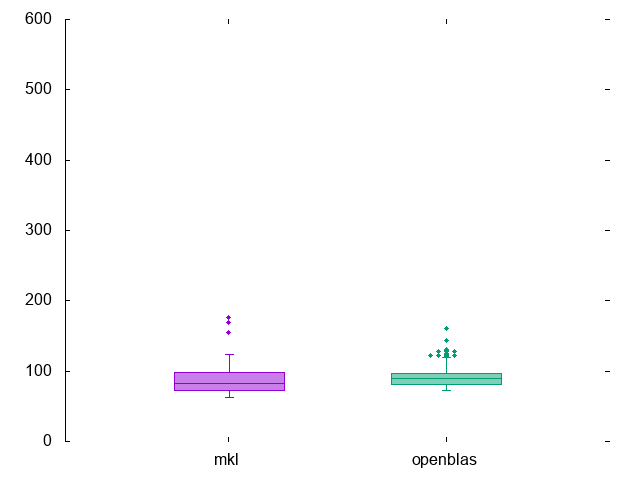
\includegraphics[width=7.5 cm]{mklVSopenblas10.png}};
\node [image,right=of frame1] (frame2) 
    {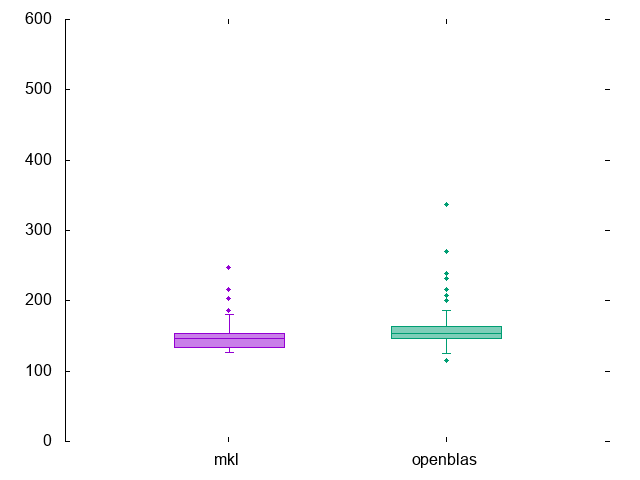
\includegraphics[width=7.5cm]{mklVSopenblas50.png}};
\node[image,below=of frame1] (frame3)
    {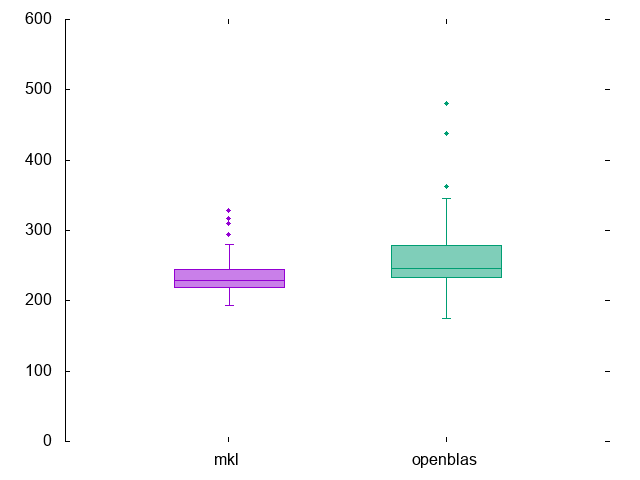
\includegraphics[width=7.5cm]{mklVSopenblas100.png}};
\node[image,right=of frame3] (frame4)
    {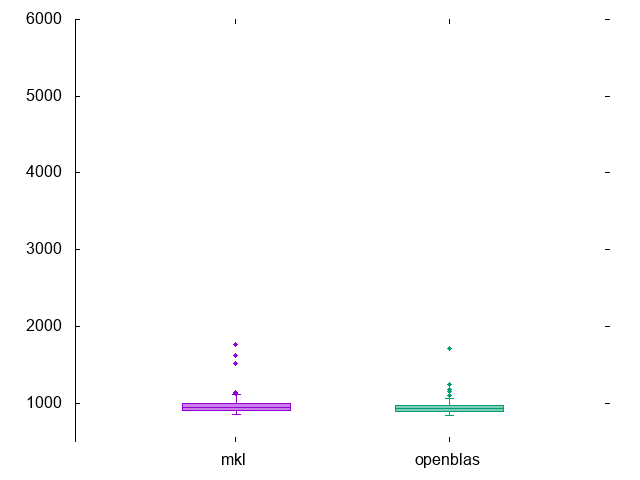
\includegraphics[width=7.5cm]{mklVSopenblas500.png}};
\end{tikzpicture}
    \caption{Starting from top left. Box plot for Matrix1 Size 10*200, 50*200, 100*200 and 500*200}
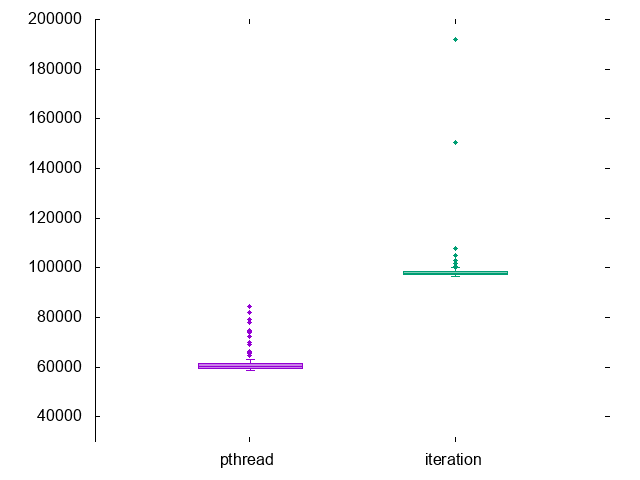
\includegraphics[width=8cm]{iterationVSpthread500.png}
    \caption{Comparison of speed between our pthread implementation and normal iterative approach for 500*200 matrix1 size }
\end{figure}


\bibliographystyle{unsrt}
\bibliography{report.bib}{}

\end{document}
